%	Predictive modelling
%
HVAD (matematisk model):
Det fremgår af AFSNIT\fxnote{ref til afsnit} at overbelægning forekommer i perioder på ortopædkirugisk afdeling. Denne rapport vil undersøge hvorvidt en prædiktiv model kan afhjælpe denne problematik. 

En prædiktiv model forsøger at forudsige hændelser med matematiske metoder eller databehandling. Med de matematiske modeller udarbejdes et ligningssystem, der kan give et muligt udfald af en fremtidig tilstand, baseret på modellens inputs. (kilde) Prædiktiv model relateres ofte til statiske metoder såsom logistiske regression og machine learning algoritmer, som automatisk kan forbedre sig selv igennem erfaring. Algoritmerne som der tales om her er neural netværk, support vector machine, decision tree og random forest. Hvis der sammenlignes mellem statiske metoder og machine learning ses det, at machine learning har den højeste nøjagtighed for en prædiktiv udsagn. (automatically exp -kilde) 

%HVOR (matematisk model):
% Examples include time-series regression models for predicting airline traffic volume or predicting fuel efficiency based on a linear regression model of engine speed versus load.




HVAD (databehandlingsmodel):
Databehandlingsmetoden varierer fra de matematiske modeller, idet der benyttes modeller, som kan være vanskelige at opstille ligninger for. Der bruges i stedet ofte simulering til at lave en forudsigelse. Denne metode kaldes også en "black box" prædiktiv model, da modellen ikke giver et indblik i, hvordan den kommer fra input til output. Der findes nogle essentielle modeller, som ikke arbejder ud fra linear, hvilket de matematiske modeller gør. Modellerne er neural netværk, support vector machines og KNN´s (K- nearst neighbors)

HVOR: 
- Neural netværk
- Support vector machine 
- KNN´s (hvis den er vigtig)

I det neurale netværk tages der udgangspunkt i et netværk af celler, hvor disse celler får input hvor de i sidste ende summerer deres givne input til en neuron, hvilket kan ses på nedenstående figur.
\begin{figure}[H]	
\centering
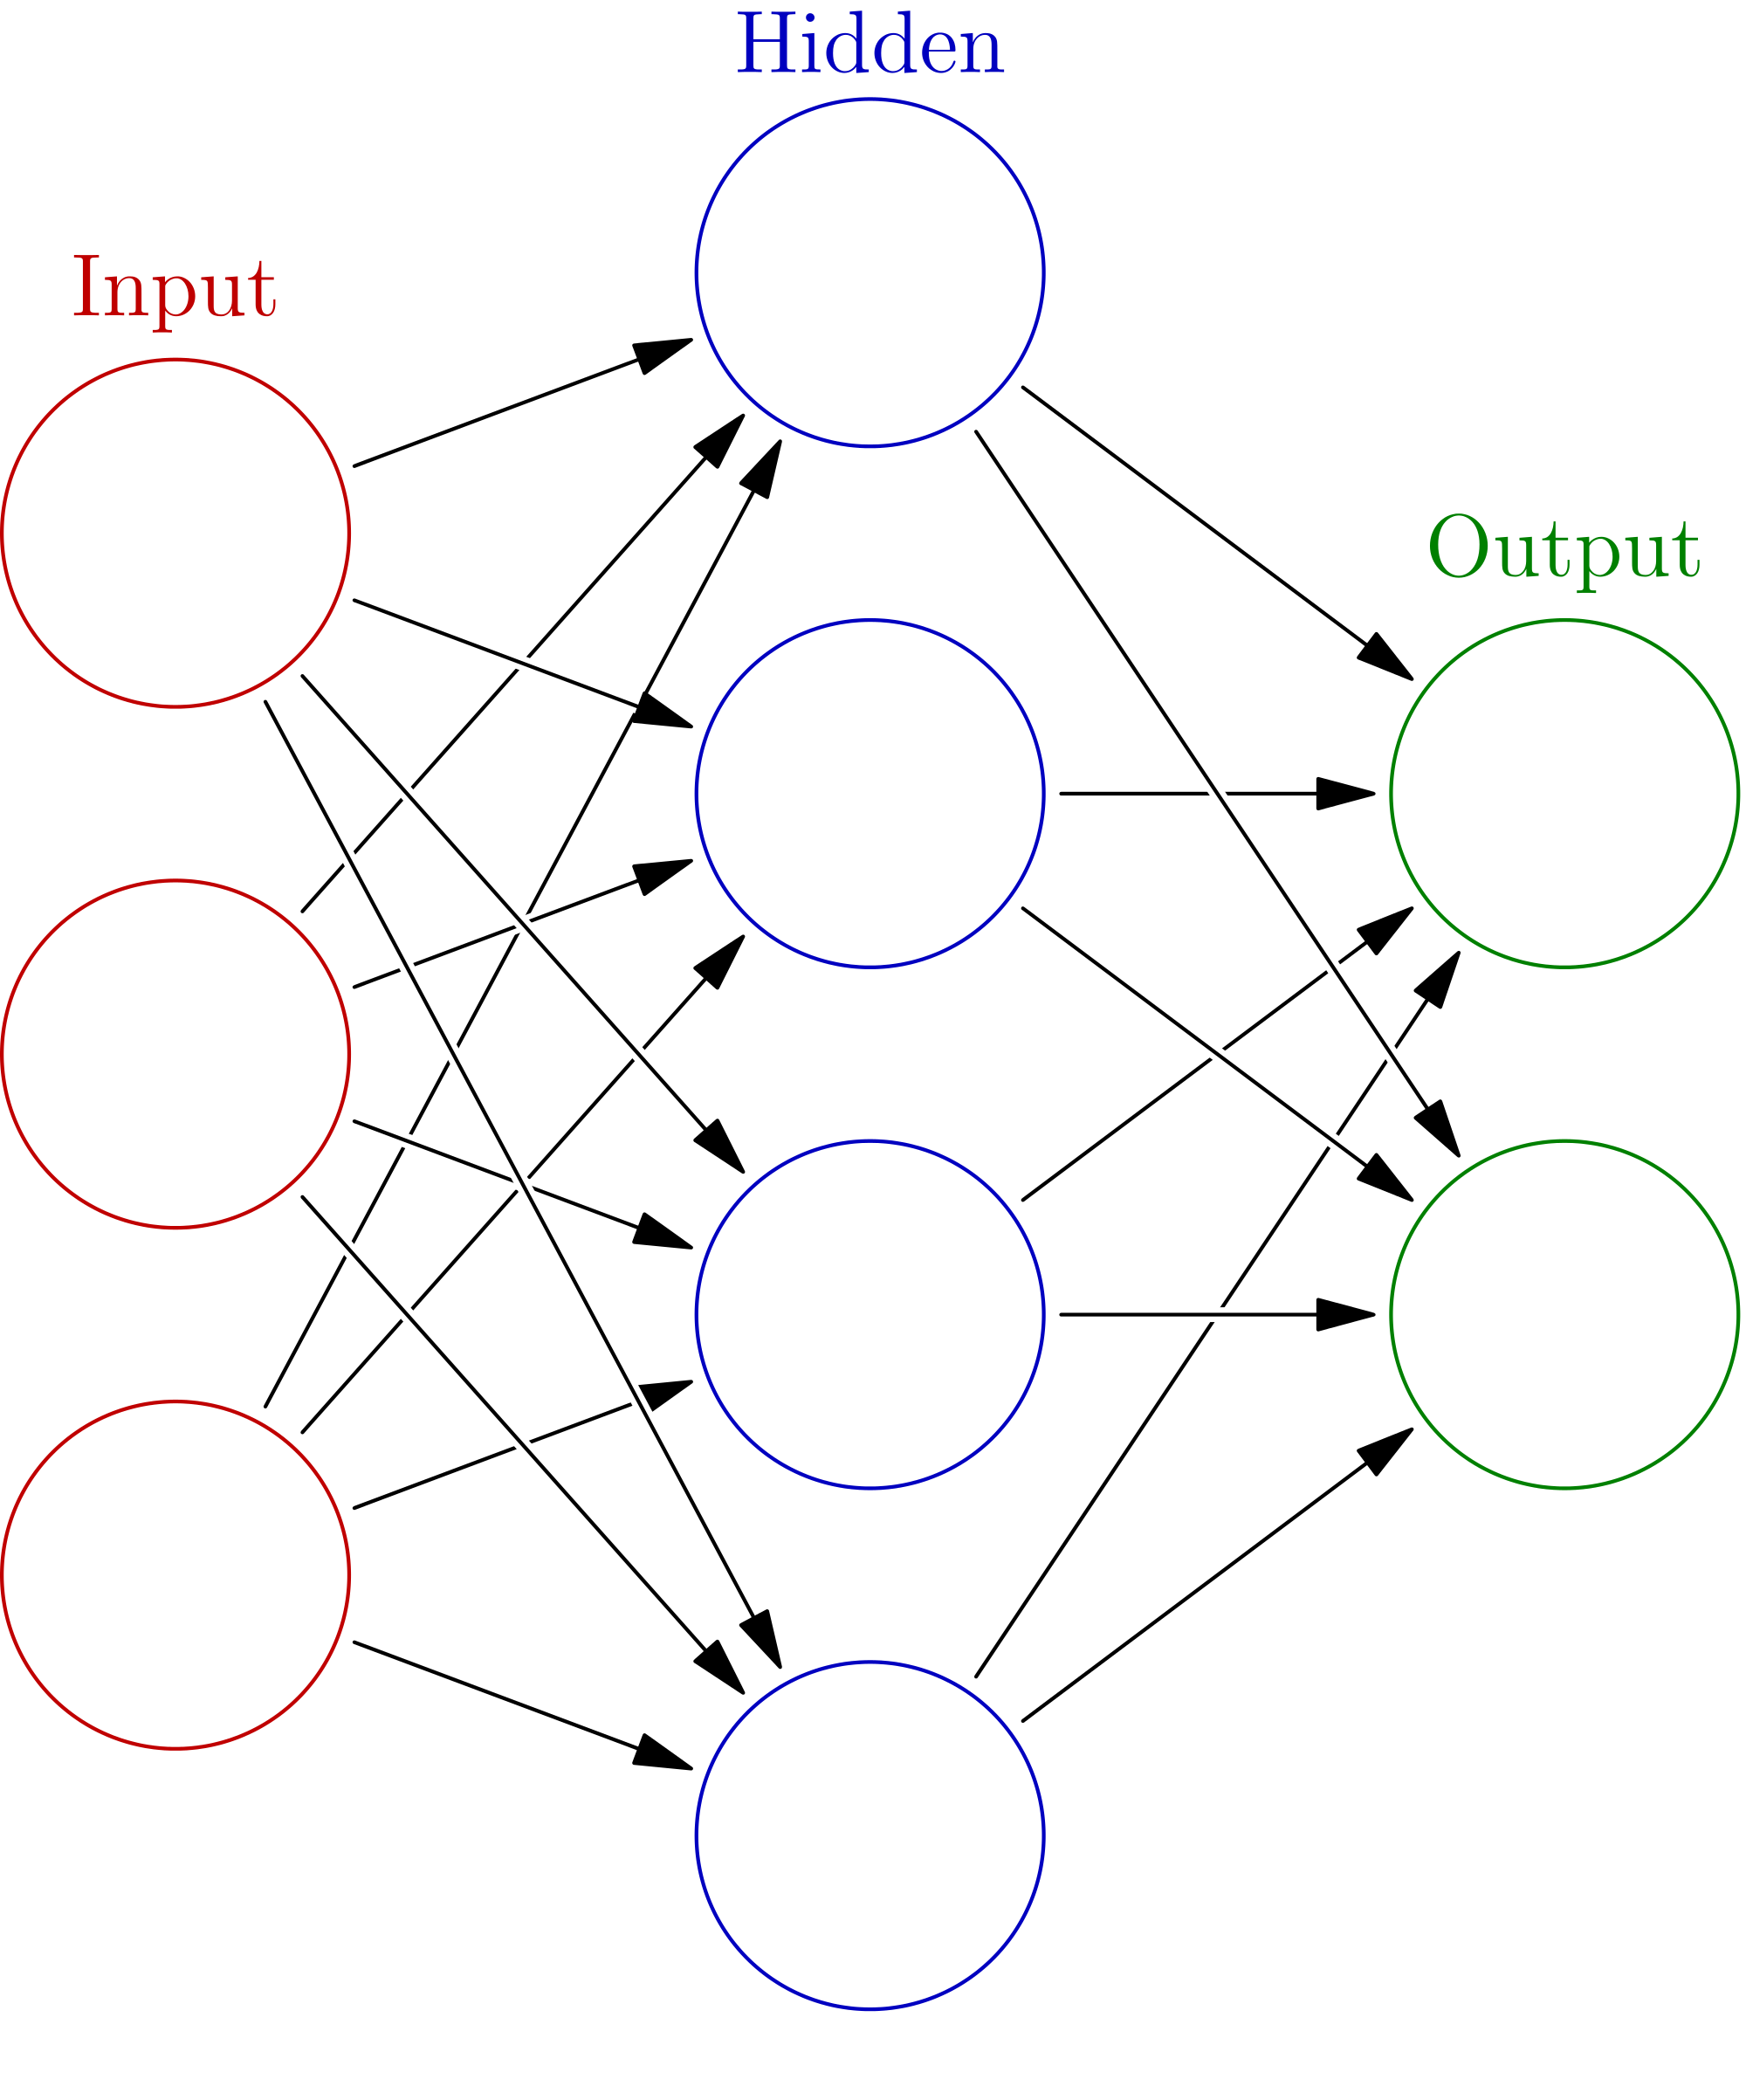
\includegraphics[width=0.5\textwidth]{fig/Neural_networkny.png}
\caption{ }
\label{fig:Neural netvaerk}
\end{figure}
Fra at cellen får et input til der fås et output fra neuroner, forgår der en proces mellem de to stadier. Processen her kaldes hidden units, der er egentlig det fundamentale og kan næsten sammenlignes med hjernen. Dataene bliver klassificeret undervejs, af de enkelte celler, hvilket betyder at netværket minimeres for fejl, samt at genereliseringsevnen vil blive stærkere. Det gælder om for netværket, at få opbygget et struktur, så den kan forudsige de aspekter den bliver spurgt ind til. \cite{DIKU2010} En af måderne netværket vil blive stærkere igennem tiden er, at den anvender begrebet feedforward netværk, der betyder at når netværket bliver anvendt bliver den trænet, samt også efter den er blevet anvendt. Dette skyldes blandt andet en mekanisme kaldt backprogproganitation.Netværket går ind og sammenligner det output den får ud sammenlignet med det der blev ønsket, og herefter kan der ud fra sammenlignings grundlaget gives feedback til de hidden units og output unitsene. (automatically exp -kilde) 

Support vector machine forsøger at udvælge nogle datapunkter, hvilket skal være med til at hjælpe løsningen. Support vector machine er også en af de algoritmer, som har den største margin og kan have det største separation mellem punkterne. En af metoderne support vector machine anvender er at den går ind og klassificere de inputs, som kommer til at ligge på dens margin, hvilket ses på nedenstående figur. 

\begin{figure}[H]	
\centering
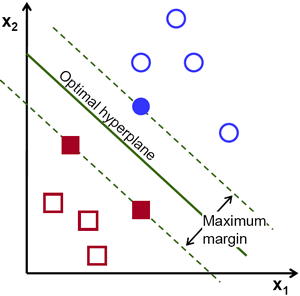
\includegraphics[width=0.5\textwidth]{fig/optimal-hyperplane.png}
\caption{ }
\label{fig:Klassifikation af inputs}
\end{figure}  

Som det ses ud fra figuren bliver der behandlet nogle data fra et træningssæt. Her ses der to forskellige elementer, som skal klassifiseres. Metoden disse elementer bliver klassificeret på er på baggrund af en hyperplane. Hyperplanens opgave er, at finde den mindste afstand til begge elementer. Der vil til at starte med blive anlagt en masse hyperplanes, men til sidst vælges hyperplanen, som er størst på marginen. Det ses udfra figuren at den optimale hyperplan er fastgjort. (Understanding machine)  




HVORDAN (begge):
% Predictive modeling is often performed using curve and surface fitting, time series regression, or machine learning approaches. Regardless of the approach used, the process of creating a predictive model is the same across methods. The steps are:

%	Clean the data by removing outliers and treating missing data
%	Identify a parametric on nonparametric predictive modeling approach to use
%	Preprocess the data into a form suitable for the chosen modeling algorithm
%	Specify a subset of the data to be used for training the model
%	Train, or estimate, model parameters from the training data set
%	Conduct model performance or goodness-of-fit tests to check model adequacy
%	Validate predictive modeling accuracy on data not used for calibrating the model
%	Use the model for prediction if satisfied with its performance



%kilde: https://se.mathworks.com/discovery/predictive-modeling.html